\documentclass[boarder=2pt]{standalone}
\PassOptionsToPackage{garamondx}{newtxmath}
\RequirePackage{newtxmath}
\usepackage{tikz}
\usepackage{garamondx}
\usetikzlibrary{%
	decorations.pathreplacing,%
	decorations.pathmorphing%
}

\definecolor{darkolivegreen}{rgb}{0.33, 0.42, 0.18}
\definecolor{darkbyzantium}{rgb}{0.36, 0.22, 0.33}
\definecolor{darkelectricblue}{rgb}{0.33, 0.41, 0.47}
\definecolor{deepchestnut}{rgb}{0.73, 0.31, 0.28}

\begin{document}
    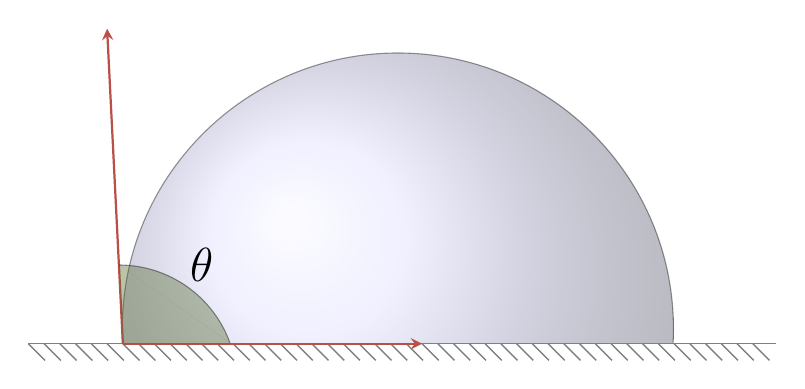
\begin{tikzpicture}[
        >=stealth,
        droplet/.style={ball color=blue!20, opacity=0.4},
         media/.style={font={\footnotesize\sffamily}},
        surface/.style={
        	postaction={draw,decorate,decoration={border,angle=-45,
        			amplitude=0.3cm,segment length=2mm}}},
        shaded/.style={
        postaction={draw,decorate,decoration={border,angle=45,
        		amplitude=0.3cm,segment length=2mm}}}
    ]


    %Draw the water droplet
    \begin{scope}
            \clip (1,1) rectangle (8.5,5);
            \draw[droplet] (4.5,1,-0.5) circle (3.5cm);
    \end{scope}
    %surface
    \draw[gray,line width=.5pt,surface](0,1)--(9.5,1);
    
    \draw[color=deepchestnut,->,thick](1.2,1)--(1,5);
    \draw[color=deepchestnut,->,thick](1.2,1)--(5,1);
    
    \draw[fill=darkolivegreen,opacity=0.4](1.15,2) arc (90:20:1.5cm);
    \fill[darkolivegreen,opacity=0.4](1.15,2)--(2.58,1,0)--(1.2,1);
    
    \node at (2.2,2) {\LARGE$\theta$};
        \end{tikzpicture}
\end{document}
